\scanpage{51}

e) Soient \deleted{$f$ une face,} $s,s',s''\in S$ formant une face $f$, et induisant \deleted{une} \inserted{par leur} ordre \deleted{opposé} une orientation de $f$ opposée de celle induite par $\Pi$ (i.e. \deleted{$s,s',s''$} si $t$ est le sommet opposé à $f$, $\rho_t$ induit \deleted{$s'=\rho_t s,\ s''=\rho_t s',$} $s\unsure{\longmapsto|\mathrel{\vdash\!\dashv}}s'\longmapsto s''\longmapsto s$) alors $(\rho_s,\rho_{s'},\rho_{s''})$ est un système de Schwartz de type $(3,3,3)$, et si $f,f',f''$ sont les faces opposées, \deleted{alors} $(\rho_{f''},\rho_{f'},\rho_f)$ est un syst. de Schwartz de type $(3,3,3)$.

\margin{$12$ syst. de Schwartz}

% slanted
\margin{\uline{NB} \deleted{\unsure{les}} \inserted{Dans un} sous-groupe de $\unsure{\mathbb H|H}\simeq\unsure{A_4|\mathcal A_4|\mathfrak A_4}$ qui soit $\ne H$ et \unsure{soit} d'ordre multiple de $3$, \deleted{\unsure{doit ê.} \illegible{1}} \deleted{\unsure{3 est} \illegible{1} d'ordre $3$} \unsure{qui} \unsure{tt les $2$ él. d'ordre $3$} \unsure{qui commutent|donc commutent}}

\margin{$12$ syst. de Schwartz}

\deleted{Les $24$} \inserted{Chacun de ces $2$ paquets de $12$} syst. de Schwartz $\{(\rho_s,\rho_{s'},\rho_{s''})\},\{(\rho_f,\rho_{f'},\rho_{f''})\}$ forment \deleted{des} une orbite sous $H$ (donc un torseur sous $H$) et leur réunion est une orbite sous $\widetilde H$ (donc un torseur sous $\widetilde H$).

% slanted
\margin{\uline{NB} les paquets de $12$ sont stables par ${\unsure{\mathfrak S_3|\mathcal S_3}}^{+}$, les \unsure{élmts} de $\mathfrak S_3^{-}$ échangent les deux paquets}

f) Les $72+24\inserted{=96}$ systèmes de Schwartz précédents de \deleted{\unsure{$A$}} $H$ sont les seuls.

\figure{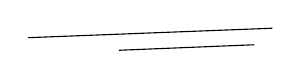
\begin{tikzpicture}[x=1cm,y=1cm]\draw (0,0) -- (3.1,.12);\draw (1.15,-.16) -- (2.87,-.09);\end{tikzpicture}}

\uline{Prouvons} f). Tout d'abord, comme les él. $\ne1$ de $H$ sont d'ordre $2$ et $3$, et que les élmts d'ordre $2$ sont contenus dans un sous-groupe inv. $V$ d'indice $2$, on voit que un syst. de Schwartz ne peut contenir deux él. d'ordre $2$, donc il contient au moins $2$ él. d'ordre $3$. \deleted{Soit $\rho,\rho',\unsure{\rho'|\rho''}$}

% archive sheet number: 50
